%!TEX root = ../../main.tex

\begin{center}
    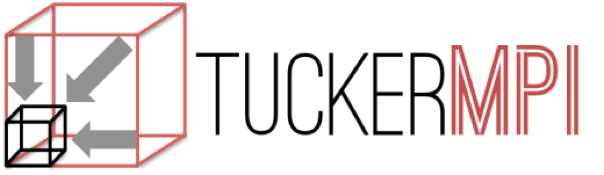
\includegraphics[scale=0.5]{/Users/joaodeoliveria/Documents/Conferences/CSE25/Figures/TuckerMPI-logo.png}
\end{center}

TuckerMPI uses $P$ processors organized into a $d$-dimensional $P_1\times \cdots
\times P_d$ grid such that $P = \prod_{i=1}^{d} P_i$ and that each processor
stores a $1/P$ fraction of $\mathcal{X}$. Our analysis will assume $\mathcal{X}
\in \mathbb{R}^{n\times \cdots \times n}$ and $\mathcal{G} \in
\mathbb{R}^{r\times \cdots \times r}$ to simplify cost comparison across
algorithms.

\subsection{TuckerMPI's STHOSVD} \label{sec:TuckerMPI's STHOSVD}
    \subsubsection{STHOSVD's Computational Complexity} \label{STHOSVD's Computational Complexity}

        The cost of LLSV in line \ref{line:sthosvd_llsv} is given by
        \begin{equation*}
            \sum_{j=1}^{d} \left(\frac{r^{j-1}n^{d-j+2}}{P} + \mathcal{O}(n^3)\right) \approx \frac{n^{d+1}}{P} + \mathcal{O}(dn^3),
        \end{equation*}
        where the first term is the cost of computing the $n \times n$ Gram matrix and
        the second term is the cost of sequentially computing the EVDs to leading order.
        %We perform the Eigendecomposition sequentially on a single processor and communicate $\Mx{U}_j$.
        After $\mathbf{U}_{k}$ is computed, $\mathcal{Y}$ is truncated by
        performing the TTM in line \ref{line:sthosvd_ttm}, which costs
        \begin{equation*}
            2\sum_{j=1}^{d} \frac{r^j n^{d-j+1}}{P} \approx 2\frac{rn^d}{P}.
        \end{equation*}
        Computing the Gram matrix is a factor of $\nicefrac{n}{2r}$ more expensive than
        the TTM and is the dominant cost for $n \gg r$. Sequentially truncating $\mathcal{Y}$
        leads to decreasing dimensions, so the algorithm is typically dominated by the
        first Gram matrix computation. Note that the EVD is not parallelized, which can
        be a barrier to parallel scaling when a single tensor dimension is large. We
        summarize the leading order STHOSVD flops cost in \cref{tab:flops} (shown in
        red).

    \subsubsection{STHOSVD's Communication Complexity} \label{sec:STHOSVD's Communication Complexity}

        TuckerMPI's parallel algorithm for LLSV explicitly forms the Gram
        matrix, $\mathbf{G} = \mathbf{Y}_{(k)}\mathbf{Y}_{(k)}^\intercal$,
        where $\mathbf{Y}_{(k)}$ is redistributed (if necessary) to a 1D column
        layout across $P$ processors, and then sequentially computes the EVD of
        $\mathbf{G}$. After redistribution of $\mathbf{G}$, each processor
        computes a local Gram matrix which can be sum-reduced (or all-reduced)
        prior to the EVD. At iteration $k$, the number of entries in
        $\mathcal{Y}$ is $r^{j-1}n^{d-j+1}$. The Gram matrix that is computed in
        each mode is of size $n \times n$, so the total communication cost is
        $dn^2$ for the all-reduce. Thus, the communication cost is given by
        \begin{equation*}
            \sum_{j=1}^{d} \bigg(\frac{r^{j-1}n^{d-j+1}}{P}\cdot \frac{P_j - 1}{P_j} + \mathcal{O}(n^2)\bigg) \approx \frac{n^{d}}{P}\cdot \frac{P_1 - 1}{P_1} + dn^2,
        \end{equation*}
        where we assume the redistribution cost is dominated by the first mode. However,
        note that there is no redistribution cost in mode $j$ if $P_j=1$. Finally, the
        parallel TTM also requires communication to perform a sum-reduce of local TTM
        results. Since the output of the TTM is largest in the first mode (of size
        $rn^{d-1}/P$), the communication cost of TTMs to leading order cost is
        \begin{equation*}
            \sum_{j=1}^{d} \frac{r^{j}n^{d-j}}{P}(P_j - 1) \approx \frac{rn^{d-1}}{P}(P_1 - 1).
        \end{equation*}
        Again, note there is no communication cost in mode $j$ if $P_j=1$.
        Because the largest data communicated occurs in mode 1, processor grids
        with $P_1=1$ are typically the fastest for STHOSVD (as we observe in our
        experiments). We summarize the STHOSVD communication costs in
        \cref{tab:comm} (shown in red).

\subsection{TuckerMPI's HOOI} \label{sec:TuckerMPI's HOOI}
    \subsubsection{HOOI's Computational Complexity} \label{sec:HOOI's Computational Complexity}

        Since HOOI is an iterative algorithm for Tucker decomposition, we analyze the
        cost of one HOOI iteration. Each HOOI iteration requires $d$ multi-TTMs, in all
        modes but mode-$j$, and $d$ LLSV computations to update factors matrices, in all
        modes. Once the factor matrices have been updated, the core tensor $\mathcal{G}$ is
        obtained by performing a TTM with the last factor matrix $\mathbf{U}{d}$. The cost
        of computing $d$ multi-TTMs is given by

        \begin{equation*}
            2d \sum_{i=1}^{d} \frac{r^i n^{d-i+1}}{P} \approx 2d\frac{rn^d}{P}.
        \end{equation*}

        The cost of each TTM decreases, so the first term in the summation (i.e. the
        first TTM) dominates. Multiplying the cost of the first TTM by $d$ yields the
        cost of $d$ multi-TTMs (i.e. one HOOI iteration). The cost of computing LLSV is
        given by
        \begin{equation*}
            d\frac{r^{d-1}n^2}{P} + \mathcal{O}(dn^3),
        \end{equation*}
        where the first term is the cost of computing the Gram matrix
        $\mathbf{Y}_{(k)}\mathbf{Y}_{(k)}'$ and the second term is the cost of
        computing the EVD. Finally, the core tensor at the end of each HOOI
        iteration is obtained by performing a TTM in mode-$d$ with the
        intermediate tensor $\mathcal{Y}$ and $\mathbf{U}_{d}$, which has a cost of
        $2\nicefrac{nr^{d}}{P}$ and is a lower order term. We summarize the
        leading order cost per HOOI iteration as implemented by TuckerMPI in
        \cref{tab:flops} (shown in red).


    \subsubsection{HOOI's Communication Complexity} \label{sec:HOOI's Communication Complexity}
        The communication cost of each iteration of HOOI is dominated by multi-TTMs and
        LLSV computations. Each TTM in the multi-TTM requires communication to perform a
        sum reduction to form $\mathcal{Y}$. Communication is required along the processor
        dimension corresponding to the mode in which a TTM is performed.
        %We consider two collectives for the sum reduction: a single reduce-scatter or $P_i$ reduces each with a different root.
        %If sufficient temporary storage is available, then a reduce-scatter is preferred as it is a factor of $2$ cheaper in bandwidth than performing $P_i$ reduces.
        %We assume that sufficient temporary storage is available and that the reduce-scatter is used.
        The size of $\mathcal{Y}$ decreases with each TTM, so the communication cost of a
        multi-TTM is dominated by the first TTM. Each HOOI iteration performs $d$
        multi-TTMs, where one iteration updates the factor matrix in the first mode.
        %We assume that the multi-TTM corresponding to $j=1$ in \Cref{alg:hooi} is performed in reverse order (starting with the mode-$d$ TTM) so that the largest TTM can be performed using a single GEMM call.
        The cost of communication for the multi-TTMs is given by
        \begin{multline*}
            \sum_{j=1}^d \bigg(\sum_{i=1}^{j-1} \frac{r^in^{d-i+2}}{P}(P_i-1) + \sum_{i=j+1}^{d} \frac{r^{i-1}n^{d-1+1}}{P}(P_i-1)\bigg) \\ \approx (d-1)\frac{rn^{d-1}}{P}(P_1 - 1) + \frac{rn^{d-1}}{P}(P_2 - 1).
        \end{multline*}
        The first term corresponds to the $d-1$ TTMs performed in the 1st mode and the
        second term corresponds to TTMs performed in the 2nd mode (for the multi-TTM in
        all but the 1st mode).
        %Each mode-$1$ TTM computes a local tensor of size $\frac{rn^{d-1}}{\Pi_{i = 2}^d P_i}$ which is reduce-scattered between processors in the $P_1$ dimension which yields a bandwidth cost of $\frac{rn^{d-1}}{P} (P_1 - 1)$ per TTM in the first mode.
        %When updating the first mode factor matrix, we perform the mode-$d$ TTM first.
        %The mode-$d$ TTM stores a local tensor of size $\frac{rn^{d-1}}{\Pi_{i = 1}^{d-1} P_i}$ which is communicated in the $P_d$ dimension.
        %Multiplying the cost of reduce-scatter in the mode-$1$ TTMs by $d-1$ and adding the cost of the mode-$d$ TTM (when $j = 1$) yields the total communication cost of multi-TTMs to leading order.

        Communication is also required when computing the LLSV in each mode.
        Using the same LLSV algorithm as in STHOSVD, the Gram matrix is computed
        in parallel followed by a sequential EVD. Computing the Gram matrix
        requires an all-to-all to redistribute $\mathbf{Y}_{(k)}$ so that it is
        stored in 1D-column layout. After redistribution
        $\mathbf{Y}_{k}\mathbf{Y}_{k}^\intercal$ is computed in parallel by
        performing local matrix-matrix multiplications that are sum-reduced to
        obtain the Gram matrix. The cost of communication for the LLSV is given
        by
        \begin{equation*}
            \frac{r^{d-1}n}{P} \sum_{i = 1}^{d}\left(\frac{P_i-1}{P_i}\right) + dn^2,
        \end{equation*}
        where the first term is the cost of all-to-all communication and the second term
        is the cost of sum reduction of the Gram matrix for one HOOI iteration (i.e. $d$
        calls to LLSV).
        %Each all-to-all requires redistribution of $\frac{nr^{d-1}}{P}$ local data which must be sent to $P_i$ processors, where $i$ is the mode in which LLSV is being computed.
        %This requires sending $P_i - 1$ messages each of size $\frac{1}{P_i} \cdot \frac{nr^{d-1}}{P}$.
        %Summing this cost over all $d$ modes yields the first term.
        %The second term is the cost of sum-reducing the $n$-dimensional Gram matrix, which has a message size cost of $n^2$ per mode.
        %Multiplying this cost by $d$ gives the second term.
        We summarize the HOOI communication costs as implemented by TuckerMPI in \Cref{tab:comm} (shown in red).


\subsection{TuckerMPI's Dimension Tree} \label{sec:TuckerMPI's Dimension Tree}
    \subsubsection{Dimension Tree Computational Complexity} \label{sec:Dimension Tree Computational Complexity}

        The flops cost of performing multi-TTMs using dimension trees is given by
        \begin{equation*}
            4 \sum_{i=1}^{d/2} \frac{r^i n^{d-i+1}}{P} + \mathcal{O} \left(d \sum_{i = d/2 + 1}^{d} r^i n^{d - i + 1}\right) \approx 4\frac{rn^d}{P},
        \end{equation*}
        where the first term is the cost of computing the TTMs in the first two branches
        (left and right of the root) in the dimension tree and the second term is the
        cost of computing the TTMs in all remaining branches. The largest TTMs in the
        first two branches dominate, so the cost of multi-TTMs is $4\cdot \nicefrac{rn^d}{P}$
        (i.e. the first TTM in each branch), which is a factor of $\nicefrac d2$ improvement over
        computing multi-TTMs directly. This cost is summarized in \Cref{tab:flops}.
    
    \subsubsection{Dimension Tree Communication Complexity} \label{sec:Dimension Tree Communication Complexity}

        Since the first TTM in each of the two multi-TTMs off the root dominate,
        the communication cost of multi-TTMs is given by
        \begin{equation*}
            \sum_{i=1}^{d/2}  \frac{r^in^{d-i-1}}{P}\left(P_i - 1 + P_{d-i+1} - 1\right) \approx   \frac{rn^{d-1}}{P} \left(P_1 + P_d - 2\right).
        \end{equation*}
        
        When traversing the right branch in the dimension tree shown in
        \cref{fig:dimtree}, TTMs are performed in the first $\nicefrac d2$ modes
        starting with mode $1$. The communication cost associated with TTMs in
        the right branch is the cost of a reduce-scatter on local data of size
        $\nicefrac{rn^{d-1}}{P}\cdot(P_1-1)$, which yields the first term. The
        second term is due to the communication cost associated with traversing
        the left branch in \cref{fig:dimtree}. TTMs in the left branch are
        performed in the last $\nicefrac d2$ modes starting with mode $d$. We
        perform left branch TTMs in reverse order because the mode $d$ TTM
        achieves higher local TTM performance due to the layout of the local
        tensor in memory. The communication cost associated with TTMs in the
        left branch is the same as the first term, except that the
        reduce-scatter is performed in the $P_d$ processor grid dimension.
        Therefore, processor grids with $P_1 = P_d = 1$ are typically the
        fastest for HOOI algorithms employing the dimension tree optimization
        (as we observe in our experiments).

        As shown in \cref{tab:flops,tab:comm}, introducing dimension trees
        memoization reduces the flops cost of TTMs in HOOI by a factor of $d/2$
        and the communication cost by a factor of $d-1$ in the first term.


\subsection{TuckerMPI's Subspace Iterations} \label{TuckerMPI's Subspace Iterations}
    \subsection{Subspace Iteration Computational Complexity.}
        Each subspace iteration requires two matrix-matrix multiplications and
        one QR decomposition. The first matrix-multiplication corresponds to the
        TTM $\mathcal{G}=\mathcal{Y} \times_k \mathbf{U}_{(k)}\intercal$ (in the
        notation of \cref{alg:Classic-HOOI}) and the second computes the tensor
        contraction $\mathbf{Y}_{(k)}\mathbf{G}_{(k)}\intercal$. The total computational cost of
        performing the TTM and contraction in each HOOI iteration is
        $4d\cdot\nicefrac{nr^d}{P}$. The cost of the QR decomposition of the
        matrix $\mathbf{Z} \in \mathbb{R}^{n\times r}$ in each HOOI iteration is
        $\mathcal{O}(dnr^2)$, where we assume a sequential QR decomposition. The
        total cost of performing subspace iteration in each mode across an
        entire HOOI iteration is given by
        \begin{equation*}
            4d\frac{nr^d}{P} + \mathcal{O}(dnr^2).
        \end{equation*}

        As shown in \cref{tab:flops}, the cost of LLSV using subspace iteration is a
        factor of $\nicefrac{1}{4} \cdot \nicefrac{n}{r}$ cheaper than the cost of LLSV via the
        Gram matrix.
        %When compared to the Gram computation in STHOSVD, HOOI with subspace iteration is a factor of approximately $\frac{1}{4dt} \cdot \prn+{\frac{n}{r}}$ faster.
        When comparing the sequential EVD to the sequential QR decomposition,
        the cost of the latter is a factor of
        $\mathcal{O}\left(\big(\nicefrac{n}{r}\big)^2\right)$ faster.
        %The best variant of HOOI based on the algorithmic improvements we have
        %introduced is HOOI with dimension trees and subspace iteration optimizations,
        %which we will refer to as HOSI-DT. \Cref{tab:flops} summarizes the flops cost
        %of $t$ iterations of HOSI-DT.

    \subsection{Subspace Iteration Communication Complexity.}
        Subspace iteration requires communication in the TTM, tensor contraction, and QR
        decomposition in each mode. The communication cost of the TTM is given by
        $\nicefrac{r^d}{P}\cdot (P_k - 1)$, where $P_k$ corresponds to the number of
        processors in the $k^\text{th}$ mode. The tensor contraction requires redistribution of
        both tensors via all-to-all communication steps. However, the all-to-all cost is
        a lower order term since it is a factor of $P_k$ cheaper than the communication
        cost associated with the TTM. Once the contraction is performed, a sum reduction
        followed by a broadcast is required to ensure that all processors can
        independently compute local QR decompositions. The communication cost of the QR
        decomposition is given by $2nr$ since $\mathbf{Z} \in \mathbf{R}^{n\times r}$ and must be
        communicated twice. As shown in \cref{tab:comm}, the total communication cost of
        the LLSV calls within an iteration of HOOI using subspace iteration is given by
        \begin{equation*}
            \frac{r^d}{P}\sum_{j=1}^{d}\left(P_j - 1\right) + 2dnr.
        \end{equation*}







\subsection{TuckerMPI's Adaptive Rank} \label{TuckerMPI's Adaptive Rank}
    \subsubsection{Core Analysis Computational Complexity} \label{sec:Core Analysis Computational Complexity}

        The cost of one RA-HOOI iteration is the same as one iteration of HOOI given in
        \cref{tab:flops}, but with the possible additional cost of performing analysis
        on the core tensor $\mathcal{G}$ to adapt the ranks for the next iteration. We solve
        the optimization problem given in \cref{eq:rankcond} exhaustively by computing
        the norm and corresponding size of every leading subtensor. This can be done
        using only $\mathcal O(dr^d)$ operations by employing a multidimensional prefix
        sum computation across the squares of the core entries. Because computational
        cost tends to be dominated by the rest of the HOOI iteration, we perform the
        core analysis sequentially, though the prefix sums are readily parallelizable.

        Assuming that this analysis is performed sequentially, the cost of the
        core analysis is $\mathcal{O}(r^d)$. The cost of the core analysis is
        dominated by the cost of computing a cumulative sum of entries in
        $\mathcal{G}$ and finding the smallest entry which meets the relative error
        tolerance. Performing these operations requires $\mathcal{O}(r^d)$
        flops. Since we need $\nicefrac nr$ to be large for HOOI to improve performance
        over STHOSVD, the cost of sequential core analysis can be performed in
        parallel, but we expect that the cost of communication would outweigh
        the benefits of parallelizing this operation.

    \subsubsection{Core Analysis Communication Complexity} \label{sec:Core Analysis Communication Complexity}

        At the end of a HOOI iteration, $\mathcal{G}$ is distributed across all processors,
        so it must be gathered on a single processor in order to perform analysis. Since
        the entire core tensor must be communicated, the all-gather cost is $r^d$ per
        HOOI iteration.
        % We opt for sequential analysis as the computation and communication costs of core analysis are low order terms when compared to the costs of TTM and LLSV.
        We demonstrate in \cref{sec:results} that the sequential cost of core analysis is typically negligible.


\begin{table*}
    \scalebox{0.862}[0.862]{
        \begin{tabular}{c|c|c|c|c|c}
            \bf Algorithm & \multicolumn{2}{|c|}{\bf LLSV} & \multicolumn{2}{|c|}{\bf TTM} & \bf Core Analysis\\ \hline\hline
            \multirow{2}{*}{\bf HOOI iteration} & \bf Gram + Eig & \textcolor{red}{$d\frac{n^2r^{d-1}}{P} + \mathcal{O}(dn^3)$} & \bf Direct & \textcolor{red}{$2d\frac{rn^d}{P}$} & \multirow{2}{*}{$\mathcal{O}(dr^d)$}\\\cline{2-5}
            & \bf Sub. Iter. & $4d\frac{nr^d}{P} + \mathcal{O}(dnr^2)$ & \bf Dim. Tree & $4\frac{rn^d}{P}$\\\hline\hline
            \bf STHOSVD & \multicolumn{2}{|c|}{\textcolor{red}{$\frac{n^{d+1}}{P} + \mathcal{O}(dn^3)$}} & \multicolumn{2}{|c|}{\textcolor{red}{$2\frac{rn^d}{P}$}} & -\\\hline
            \bf RA-HOSI-DT & \multicolumn{2}{|c|}{$\ell\left(4d\frac{nr^d}{P} + \mathcal{O}(dnr^2)\right)$} & \multicolumn{2}{|c|}{$\ell\left(4\frac{rn^d}{P}\right)$} & $\ell \left(\mathcal{O}(dr^d)\right)$\\\hline
        \end{tabular}
    }
    \caption{Leading order flops costs of LLSV (Gram + Eig and Subspace Iteration), multi-TTM (Direct and Dimension Trees) and Core Analysis algorithmic choices for HOOI and a comparison between STHOSVD and HOOI with Subspace Iteration and Dimension Trees (HOSI-DT) optimizations. We assume $\ell$ iterations of HOSI-DT are performed.}
    \label{tab:flops}
\end{table*}

\begin{table*}
    \scalebox{0.62125}[0.8]{
        \begin{tabular}{c|c|c|c|c|c}
            \bf Algorithm & \multicolumn{2}{|c|}{\bf LLSV} & \multicolumn{2}{|c|}{\bf TTM} & \bf Core Analysis\\ \hline \hline
            \multirow{2}{*}{\bf HOOI iteration} & \bf Gram + Eig & \textcolor{red}{$\frac{nr^{d-1}}{P}\sum_{i=1}^{d}\frac{P_i-1}{P_i} + dn^2$} & \bf Direct & \textcolor{red}{$(d-1)\frac{rn^{d-1}}{P}(P_1 - 1) + \frac{rn^{d-1}}{P}(P_2 - 1)$} & \multirow{2}{*}{$r^d$}\\\cline{2-5}
            & \bf Sub. Iter. & $\frac{r^d}{P}\sum_{i=1}^{d} \left(P_i - 1\right) + 2dnr$ & \bf Dim. Tree. & $\frac{rn^{d-1}}{P}(P_1 - 1) + \frac{rn^{d-1}}{P}(P_d - 1)$\\\hline\hline
            \bf STHOSVD & \multicolumn{2}{|c|}{\textcolor{red}{$\frac{n^d}{P}\frac{P_1-1}{P_1} + dn^2$}} & \multicolumn{2}{|c|}{\textcolor{red}{$\frac{rn^{d-1}}{P}(P_1 - 1)$}} & -\\\hline
            \bf RA-HOSI-DT & \multicolumn{2}{|c|}{$t\Big(\frac{r^d}{P}\sum_{i=1}^{d} (P_i - 1) + 2dnr\Big)$} & \multicolumn{2}{|c|}{$t\Big(\frac{rn^{d-1}}{P}(P_1+P_d-2)\Big)$} & $\ell \left(r^d\right)$\\\hline
        \end{tabular}
    }
    \caption{Leading order bandwidth costs of LLSV (Gram + Eig and Subspace Iteration), multi-TTM (Direct and Dimension Trees) and Core Analysis algorithmic choices for HOOI. For reference, we include a comparison between STHOSVD and HOOI with Subspace Iteration and Dimension Trees (HOSI-DT). We assume a processor grid of $P = (P_1\times \cdots \times P_d)$ and that $\ell$ iterations of HOSI-DT are performed.}
    % \AD{consider removing factors of $1 - 1/P_i$ for STHOSVD and HOOI to simplify the table, since these are easy to upper bound. Sub. iter. is a diverging series, so harder to simplify.}
    \label{tab:comm}
    % \AD{I think HOOI Gram+Eig and Sub. Iter. costs need a factor of $\sum_{i = 1}^{d} \frac{P_i - 1}{P_i}$ in the Gram bandwidth term.}
    % \AD{HOOI TTM cost implies that the mode-$1$ factor matrix is resized to the new rank. However, if $r$ increases then we do not increase size of $\Mx{U}{1}$. The asymptotic cost stays the same, but doesn't accurately capture our implementation. Also, if we assume that modes are processed in natural order then I think the next largest TTM cost should be $P_2$ and not $P_d$?}
\end{table*}